\chapter{Algorithm}
\label{chapter:algorithm}

After meticulous research on behaviour and abilities of \textit{Physarum Polycephalum} and acquaintance of Quadratic Assignment Problem field knowledge, we could proceed with design of the new algorithm. Initial concept assumed creating a Physarum Machine --- a method of computation made directly on the slime mould, where inputs are defined by positions of food sources and physical constrains and results can be read via interpretation of slime mould's movements and other behaviours.

Such machine requires specific placement of food sources and constraints which must be transformed from QAP input into positions on physical Petri dish surface. Initial positions of \textit{Physarum} colonies must be declared too. When environment for the experiment is created, scrupulous observations of foraging plasmodium must be continously made --- one can use human observer or automate this process using a camera and image processing software. During the experiment input can be modified if the algorithm requires such step. In the end solution for the QAP can be distilled from the observations. General schematic for universal physarum machine is given on figure \ref{figure:a_machine}.

\begin{figure}
  \centering
  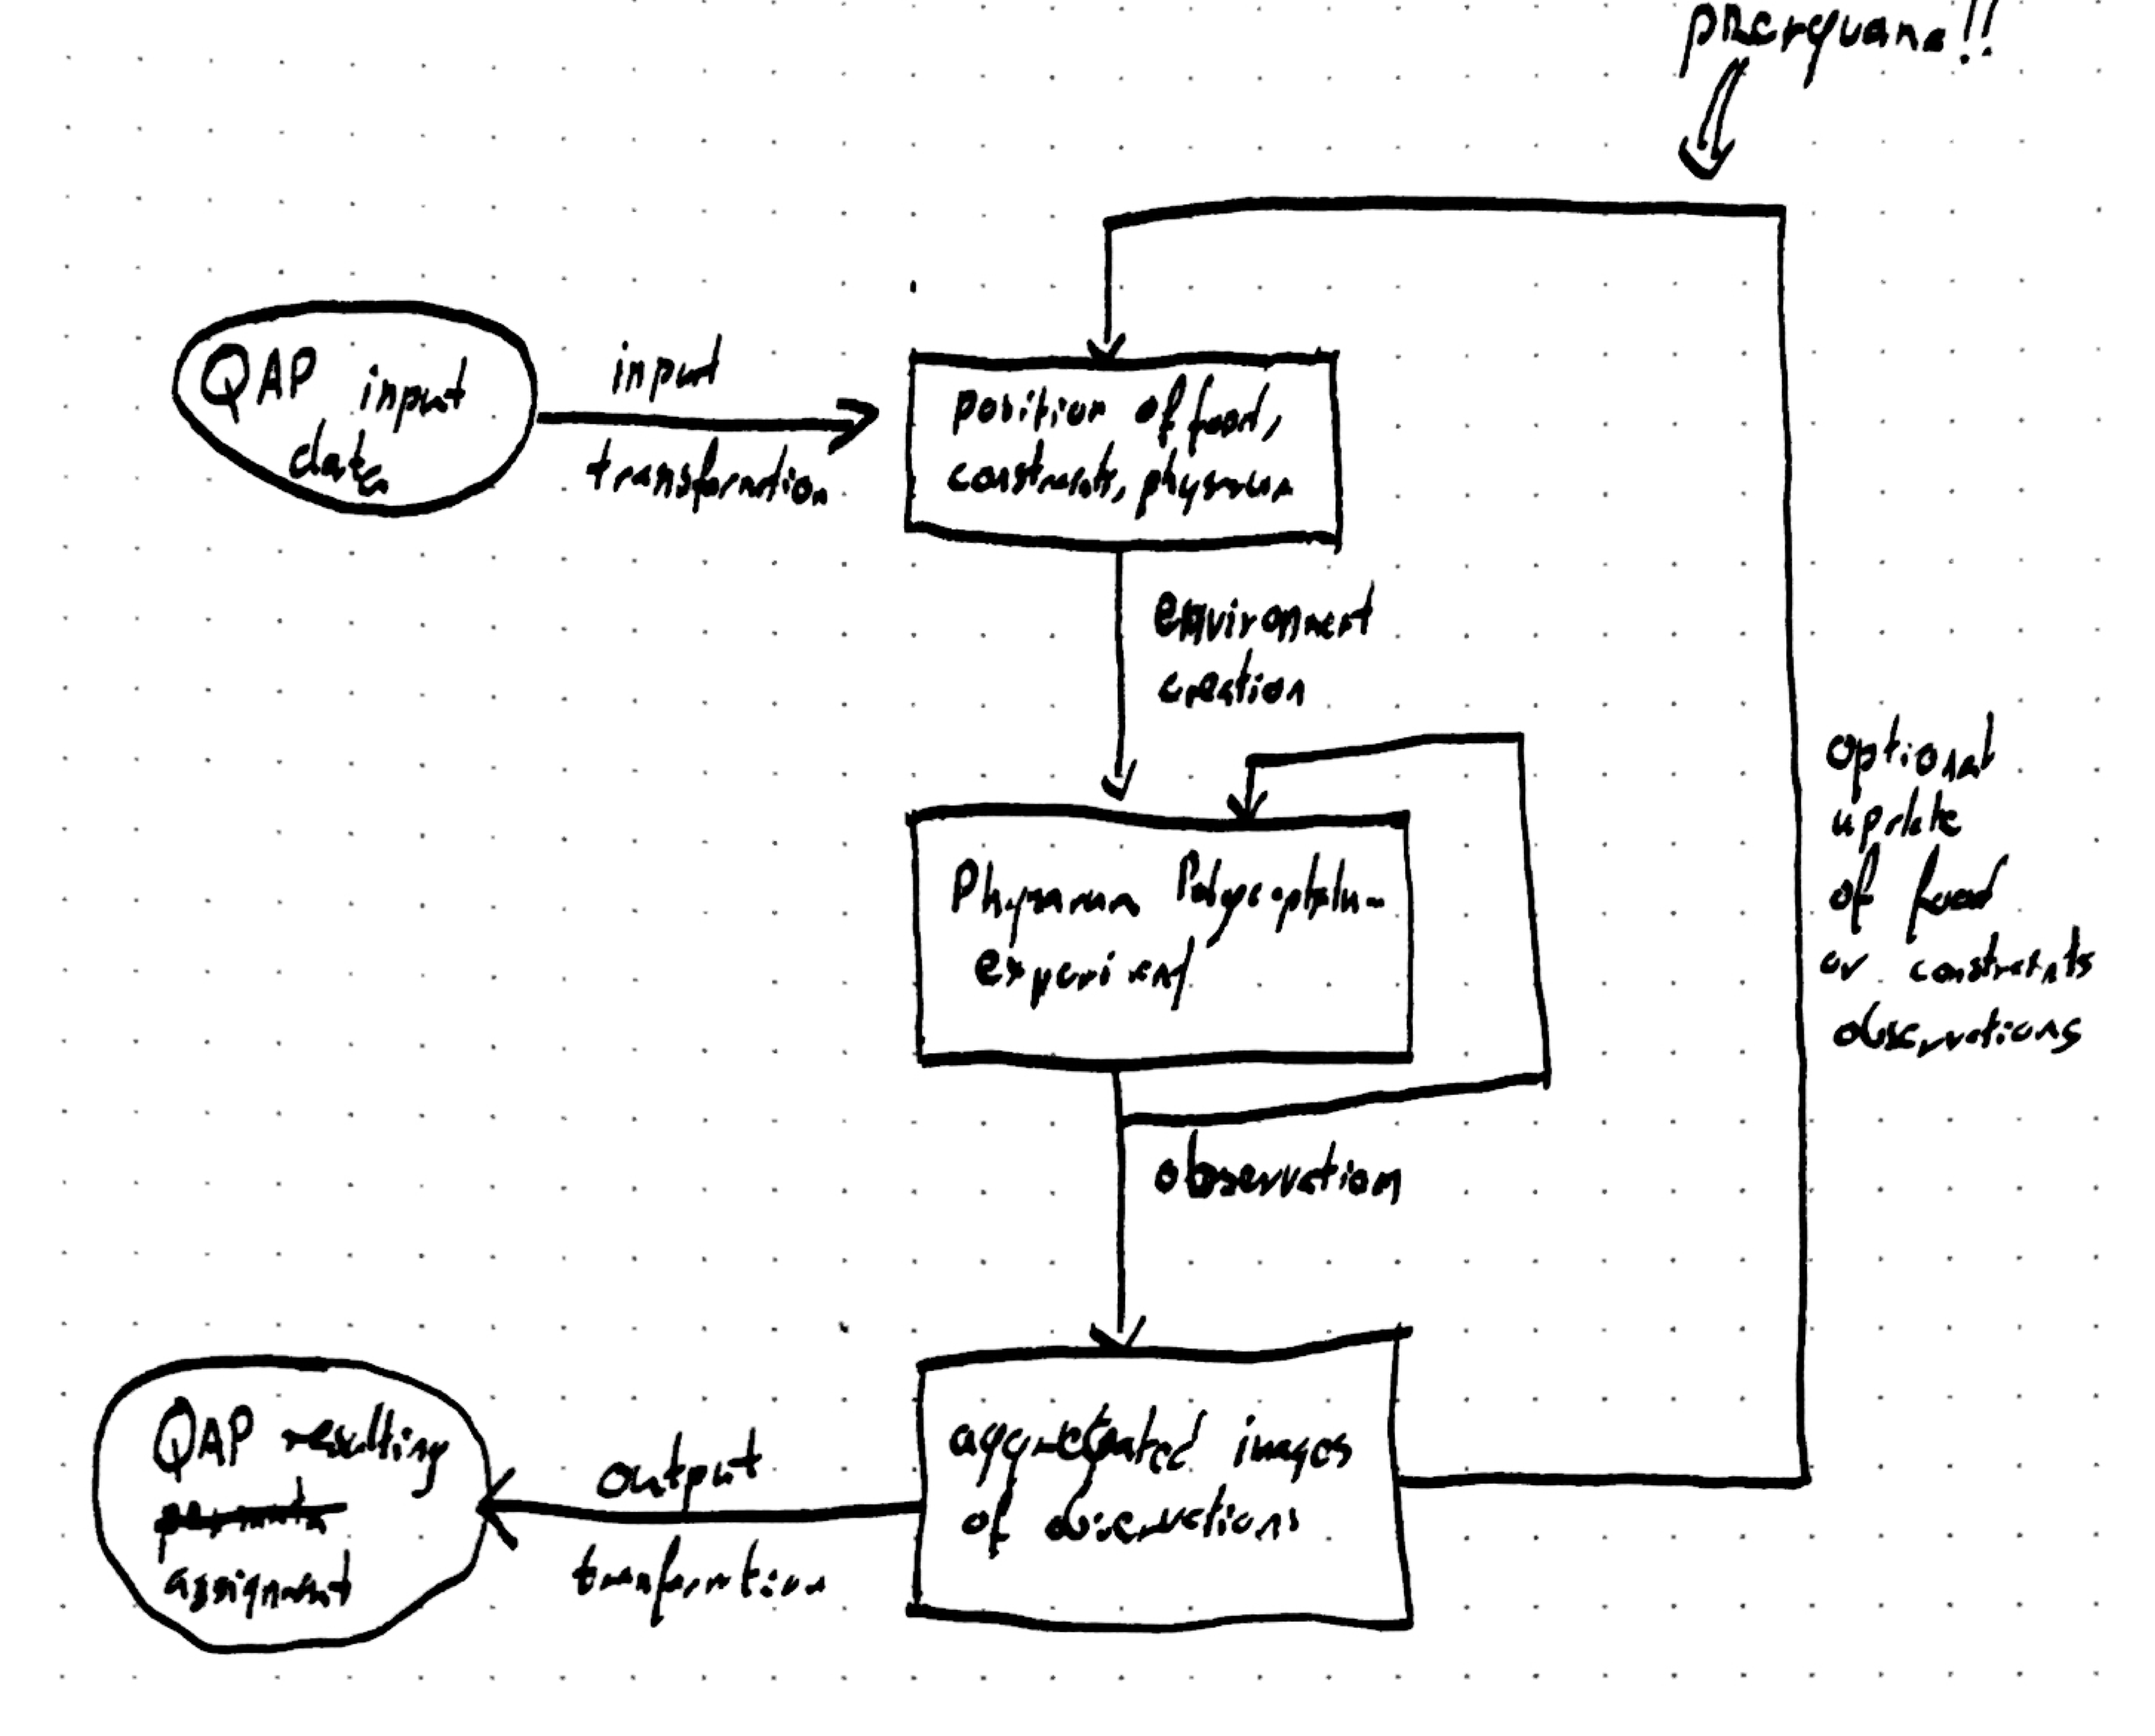
\includegraphics[width=0.84\textwidth]{algorithm/physarum_machine.png}
  \caption{Generic physarum machine schematic}
  \label{figure:a_machine}
\end{figure}

It can be seen that design of the Physarum Machine is a complex task --- methods of communication, observation, food placement, limits formation must be created, not to mention essential two non-trival transformations must be engineered. Quadratic Assignment Problem is defined by two input matrices --- weight matrix and distance matrix. While it is natural to interpret weight matrix as graph of facilities connected with trade relation, one cannot think the same about the location matrix since it depends on the assignment: one of interpretions of the problem is to assign these facilities so transport cost of goods between different facilities is the lowest. Finding the optimal assignment is a complex task, in fact there are $n!$ possible assignments. As previously shown slime moulds have been used to approximate solutions of some graph problems (such as shortest path or networking problem), there are even some approaches to solving Travelling Salesman Problem --- all of these issues have one thing in common, stating the problem in \textit{Physarum} domain, as set of food locations and constraints is trivial as \textit{input transformation} is relatively easy function. 

An obvious challenge is to model QAP input using a \textit{input transformation function}, only when such function is defined, the other part of the machine, \textit{output transformation function} can be designed. The \textit{output transformation} could use movement of plasmodium, oscillations of pseudopodia or other observations to obtain the solution, the final assignment.

Initially we thought of treating the slime mould as restricted linear programming solver, stating the QAP in one of the forms of linearized mathematical programming problems. Literature gives many different approaches for such linearization, but even these did not inspire us for any practical representation in a "slime mould world". There is some research on stating QAP as various graph problems \cite{cela2013quadratic}, but we have not genuinely explored this path. Another approach has been proposed, which explores space of all possible assignments using crawling plasmodium. It could have been implemented as physical physarum machine, however it have no practical benefits, requiring lots of preparation and observation overhead. Details of this algorithm are presented it the next section. While it may not be practical, it showed us that we are not capable of designing a better physarum machine, however we took an inspiration from this experience and designed a metaheuristic based on observed behaviour of \textit{Physarum Polycephalum}.

\section{Naive Space Search using Physarum Polycephalum}
\label{section:algorithm_naive}

Using classic definition of Quadratic Assignment Problem, we can assign a cost $c : f \rightarrow \mathbb{R}$, $c(f) = \sum_{a,b\in P}w(a,b)\cdot d(f(a), f(b))$ for each assignment $f$. The goal is to find assignment minizing the cost. To approximate the solution, we propose variation of brute force algorithm implemented as a Physarum Machine.

The input transformation is rather simple: for each possible $n!$ assignments we compute its cost and transform it to size of food source using examplar function $g(c(f)) = \frac{a}{q^{c(f)+k}}+b$, where $a$ and $k$ are scaling factors and $b$ is bias, the exponential function of base $q$ is used to amplify small costs. The parameters of function $g$ can be selected in such manner that small difference in cost is represented by not-so-small difference in food source mass. Food sources of weight proportional to $g(c(f))$ made of porridge (sterile oatmeal paste) are placed uniformly on the substrate --- for each assignment there is a respective food source with its size exponentially inversely proportional to the cost. Number of the slime mould colonies in plasmodial stage are placed on this prepared environment. Now observations could be made --- the experiment proceeds as long as plasmodium actively moves within given observation timeframe. 

Exploiting the fact that \textit{Physarum Polycephalum} prefers to consume the biggest food source, an output transformation simply takes position of the plasmodium and returns an assignment linked with physical food source where the plasmodium resides. It should be remembered that the slime mould is a living creature and results obtained using this algorithm are just an approximation as plasmodium behaves nondeterministically when foraging.

Presented algorithm is just a concept and has not been tested in a wet lab as it is highly unpractical. The input transformation requires computing food size for every possible $n!$ assignment, then a human or CNC must place this food on a substrate (which itself must be big enough to contain everything), then long, many days observations must be done until the plasmodium stops crawling. With that much work, we would get only an approximation --- the approximation of $argmin$ function which could have been worked out using a computer giving accurate results, probably in time shorter than time needed for computing the input transformation. Usage of such physarum machine gives no additional quality --- obtained result is just an approximation calculated in longer time than basic exhausitive brute force which gives an optimal assignment. While it was an educational experience, we conclude that we are not able to create a physarum machine for solving QAP working in reasonable time with reasonable results.


\section{Physarum-based Metaheuristic}
\label{section:algorithm_metaheuristic}

foo bar

